\documentclass[10pt,a4paper]{article}
\usepackage[utf8]{inputenc}
\usepackage{graphicx}
\usepackage{listings}

\author{Kim Rostgaard Christensen}
\title{Tool-assisted verification and validation}


\begin{document}
\maketitle

\abstract{With the increasing complexity, the need for a formalized approach to verification and validation becomes apparent to document activities, and make them traceable.}

\tableofcontents
\newpage

\section{Introduction}
This report used the EN-50126 standard for railways as the formal process to implement. As the EN-50126 contains a very general approach to V\&V, the methods discussed here should be applicable elsewhere.

%Unified Modelling Language (UML) is discussed in this report. Version 1 of UML is implied, but the current version is 2.0.
\subsection{Background}
I was noted that the challenges of the development process of a larger software project, and the challenges


\subsection{Terminology of EN-50126}
The EN-50126 defines a number of phases and activities

\subsection{Terminology of software project management}
Typically you have a hierarchy consisting of projects, subprojects and components. The structure is illustrated in figure \ref{fig:project_structure}.

\begin{figure}[h]
\centering
%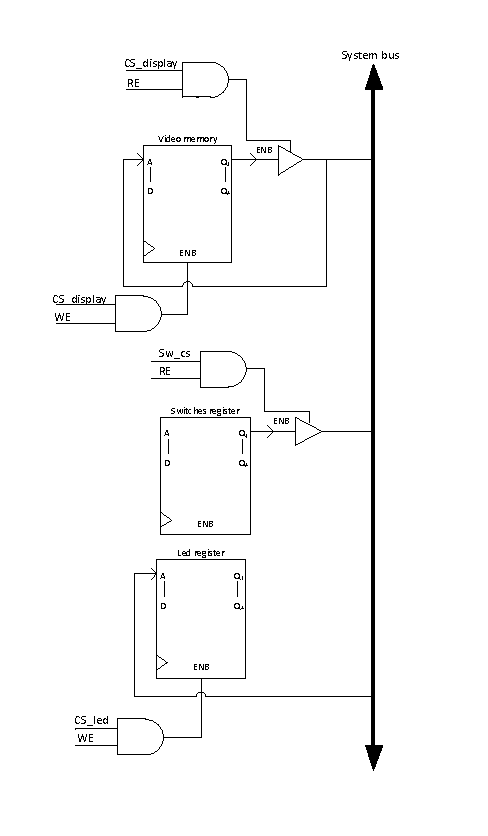
\epsfig{file=fig/system.eps, width=3.0in}
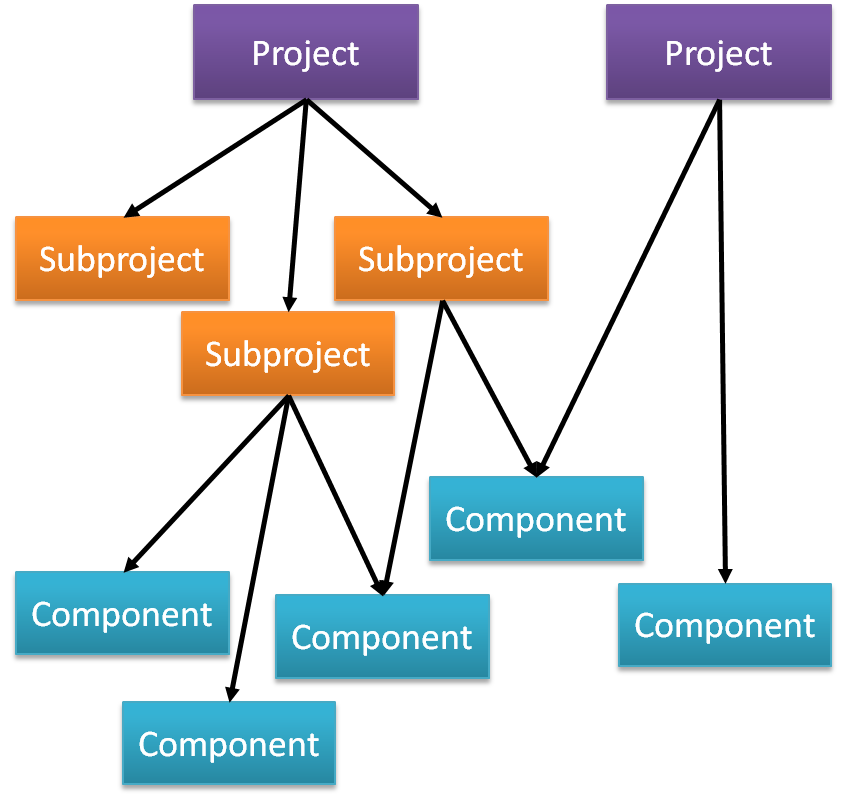
\includegraphics[scale=0.6]{fig/project_structure.png} 
\caption{Software project structure}
\label{fig:project_structure}
\end{figure}

TODO: The need for 


\subsubsection{Issues}
A software issue is often also referred to as a bug, for historical reasons.
The lifecycle of a bug is shown in figure 


\begin{figure}[h]
\centering
%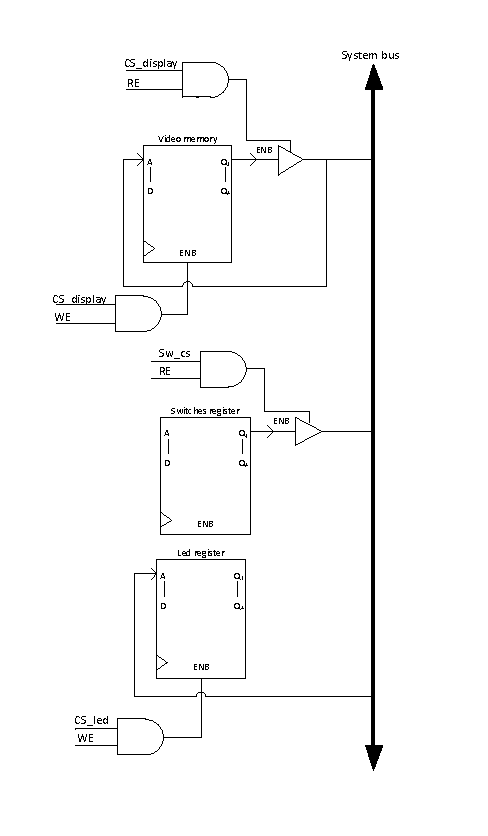
\epsfig{file=fig/system.eps, width=3.0in}
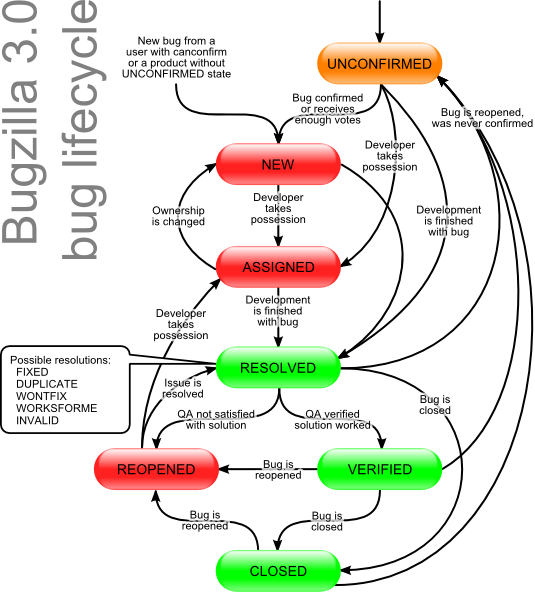
\includegraphics[scale=0.45]{fig/Bugzilla_Lifecycle_color-aqua.png} 
\caption{Life cycle of a software issue}
\label{fig:software_issue_life_cycle}
\end{figure}


\section{Mapping}
Freezing 

\section{Discussion}
The main motivation and goal for using a tool in the V\&V process must be to eliminate tedious low-practical tasks, and unify the parts of the validation process that allows it.

The tasks can include an automatic header generator filling out the revision log with the information provided by the validator.

What it is not:
It is not a strict system that decides what format your document must be written in.

\section{Events}
\subsection{Quality assurance}

\subsection{Validation}
A validation starts by appointing a validator. This is done by any document author.

The validator will then receive access to the validation view of the document management system.


\section{Notes}
Qualifications of persons can be asserted by their profile, with an import functionality to, as of this writing, a de facto CV database such as Linkedin\footnote{http://linkedin.com}. Or, an attached pdf file.


%\section{UML}
%In software engineering there exists a semi-formal language for real-world modelling. It is not based on any character-based language, as you may expect , but instead on diagrams and descriptions. This has the great advantage, that the process of mutual agreement across professions, ideally, becomes easier.
%
%This is a bold statement. And in order to demonstrate, the following sections will give examples on usage
%\subsection{Diagram types}
%The backbone of UML is its extensive use of graphical representation of a real-world scenario. 
%
%\subsection{Use cases}
%A simple example can be seen in figure \ref{fig:use_case_diagram_example}.
%\begin{figure}[h]
%\centering
%%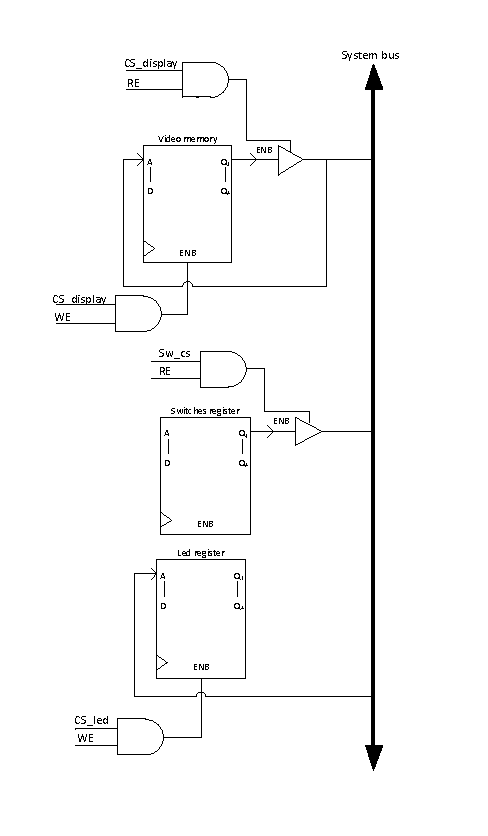
\epsfig{file=fig/system.eps, width=3.0in}
%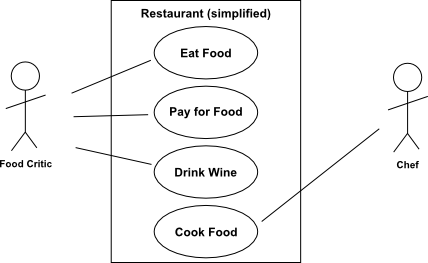
\includegraphics[scale=0.6]{fig/UML_Use_Case_diagram.png} 
%\caption{Use Case Diagram example}
%\label{fig:use_case_diagram_example}
%\end{figure}
%
%\subsection{State diagrams}
%\begin{figure}[h]
%\centering
%%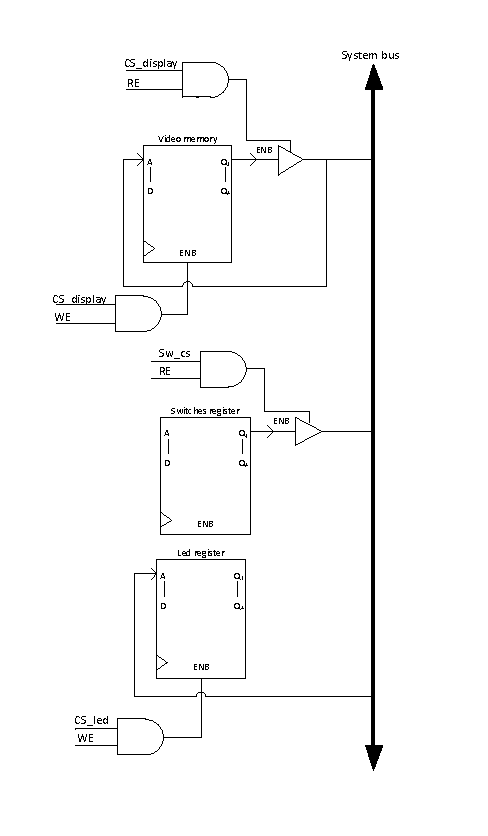
\epsfig{file=fig/system.eps, width=3.0in}
%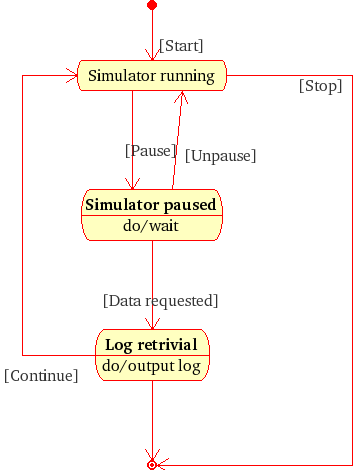
\includegraphics[scale=0.45]{fig/UML_state_diagram.png} 
%\caption{State Diagram example}
%\label{fig:state_diagram_example}
%\end{figure}
%
%The state diagram is also widely used in digital electronics.
%
%
%\subsubsection{Sequence diagrams}
%
%\subsubsection{Other types}
%
%
%\subsubsection*{Flow diagrams}
%Though strictly not a part of UML, classic flow diagrams are a good addition to use case diagrams.
%
%
%\subsection{Discussion}
%The main advantage of UML is primarily found in the software engineering field - and from this perspective. However, it has proved itself to be a very powerful communication tool, when work-flow and logic has to be modelled in software.
%
%Applying some of the techniques to other engineering disciplines can, potentially, provide benefits - but is also liable to the common pitfalls of trying using tool in a way it was not intended to be used.
%
%UML is subject to continuous critique from the software engineering field, and these points should be taken into consideration in an adoption.
%\section{Project management examples}
%A lot of time, work and money can be saved if an existing software management tool is converted to a specialized EN-50126 tool.
%
%This section is meant as a brief description of some of the existing tools available.
%\subsection{Bugzilla}
%Bugzilla has been around since the 
%
%\subsection{Tracks}
%Tracks implement the Getting Things Done methodology\footnote{TODO}. Which is a simplistic approach to put a system to relatively sporadic ideas and tasks continuously. It is also project oriented, but is more dynamic in nature.
%
%\subsection{Redmine}
%Redmine is a more full-featured project management tool.
%

\appendix
\section{Figures}
\listoffigures

\end{document}